\documentclass[12pt]{article}

\usepackage[margin=1in]{geometry}
\usepackage{amsmath,amsthm,amssymb}
\usepackage{graphicx}

\newcommand{\N}{\mathbb{N}}
\newcommand{\Z}{\mathbb{Z}}

\newenvironment{theorem}[2][Theorem]{\begin{trivlist}
\item[\hskip \labelsep {\bfseries #1}\hskip \labelsep {\bfseries #2.}]}{\end{trivlist}}
\newenvironment{lemma}[2][Lemma]{\begin{trivlist}
\item[\hskip \labelsep {\bfseries #1}\hskip \labelsep {\bfseries #2.}]}{\end{trivlist}}
\newenvironment{exercise}[2][Exercise]{\begin{trivlist}
\item[\hskip \labelsep {\bfseries #1}\hskip \labelsep {\bfseries #2.}]}{\end{trivlist}}
\newenvironment{problem}[2][Problem]{\begin{trivlist}
\item[\hskip \labelsep {\bfseries #1}\hskip \labelsep {\bfseries #2.}]}{\end{trivlist}}
\newenvironment{question}[2][Question]{\begin{trivlist}
\item[\hskip \labelsep {\bfseries #1}\hskip \labelsep {\bfseries #2.}]}{\end{trivlist}}
\newenvironment{corollary}[2][Corollary]{\begin{trivlist}
\item[\hskip \labelsep {\bfseries #1}\hskip \labelsep {\bfseries #2.}]}{\end{trivlist}}

\newenvironment{solution}{\begin{proof}[Solution]}{\end{proof}}

\begin{document}

\title{Review Questions 1}
\author{Group 1 \\ Chuan Su \\ Diego Alonso Guillen Rosaperez}

\maketitle
\begin{enumerate}
	\item All of these three statements are true about \textit{Normal Equation}.
	\begin{enumerate}
\item We don’t have to choose the learning rate.
\item It becomes slow when number of features is very large.
\item No need to iterate.
	\end{enumerate}
\item $SSE = (-0.2)^2 + (0.4)^2 + (-0.8)^2 + (1.3)^2 + (-0.7)^2 = 3.02$
\item \texttt{a} and \texttt{d} are correct.
\begin{enumerate}
\item[(a)] In case of fewer observations, it is easy to overfit the data.
\item[(d)] In case of more observations, it is hard to overfit the data.
\end{enumerate}

\item Two coefficients - $w_0$ and $w_1$ for $y = w_1*x + w_0$
\item \textit{Cross-validation} is a technique useful for ensuring the effectiveness of a model, specially by mitigating overfitting. The training set is split into complementary training and validation subsets. Each model is trained against a different combination of these subsets and validated against the remaining parts. Once the model type and hyperparameters have been selected, a final model is trained using these hyperparameters on the full training set, and the test error is measured on the test set.

\item
\textit{Sigmoid}:
\[p1 = sigmoid(\theta h) = \frac{1}{1+e^{-\theta h}}\]
\[p2 = 1-sigmoid(\theta h) = \frac{1}{1+e^{\theta h}}\]

\textit{Softmax} $k=2$:

\[p1 = \frac{e^{\theta_1 h }}{e^{\theta_1 h} + e^{\theta_2 h } } = \frac{1}{1 + e^{(\theta_2-\theta_1) h}}\]
\[p2 = \frac{e^{\theta_2 h }}{e^{\theta_1 h} + e^{\theta_2 h } } = \frac{1}{1 + e^{(\theta_1-\theta_2)h}}\]

\textit{Given}  $\theta = \theta_1 - \theta_2$, \textit{softmax} function is equivalent to the \textit{sigmoid} function with two classes.

\item  \texttt{-log} ensures convexity of logistic regression cost function and convergence to a global minimum. Moreover, with \texttt{-log}  the cost function output closes to 0 if the predicted value y is close to true values and large if the predicted value y is far from the true value.

\item 
\begin{enumerate}
	\item Cross-entropy and negative log-likelihood are the probabilistic interpreatation of the logistic regression cost function.
	\item The equation of negative log-likelihood is the same as the logistic regression cost function. Therefore minimize the negative log-likelihood is to minimize the logistic regression cost fucntion.
	\item Negative log-likelihood is also called cross-entropy, which is the logistic cost function. Cross-entropy quantify the difference (error) between the predicted distribution and the true distribution. Minimize the cross-entropy is to minimize the logistic regression cost function.
\end{enumerate}

\item The receiver operating characteristic (ROC) curves summarize the trade-off between True Positive Rate (TPR) and False Positive Rate (FPR) for a model at different probability thresholds. Lowering the threshold classifies more items as positive, thus increasing both True Positive and False Positive. The higher the TPR is, the more FPR the classifier produces. To compute the points in an ROC curve, we need to evaluate the classification model, i.e. a logistic regression, many times with different threshold values.

$ TPR=\frac{TP}{TP + FN} $ and $ FPR=\frac{FP}{FP + FN} $

\begin{figure}[h]
	\centering
	\scalebox{0.4}{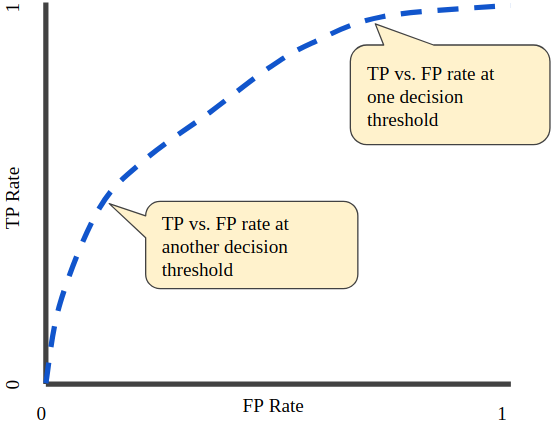
\includegraphics{rocCurve.png}}
	\caption{ROC curve from Google Developers}
\end{figure}
Google Developers: https://developers.google.com/machine-learning/crash-course/\\
classification/roc-and-auc
\end{enumerate}
\end{document}
